\documentclass[tikz,border=2pt]{standalone}
\usepackage{amsmath,amssymb}
\usepackage{tikz}
\usetikzlibrary{arrows.meta}

\begin{document}
% An iterative algorithm: a fixed rule is applied repeatedly from a starting point until a
% stopping condition certifies the answer (simplex pivots, label settings, DP stages).
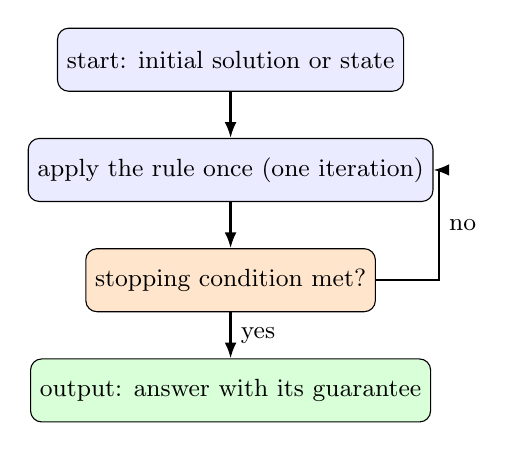
\begin{tikzpicture}[every node/.style={font=\small}, >={Latex[length=2mm]}, b/.style={draw, rounded corners=4pt, minimum width=3.6cm, minimum height=8mm, fill=blue!8, align=center}]
	\node[b] (s) at (0,0) {start: initial solution or state};
	\node[b] (it) at (0,-1.4) {apply the rule once (one iteration)};
	\node[b, fill=orange!20] (q) at (0,-2.8) {stopping condition met?};
	\node[b, fill=green!15] (o) at (0,-4.2) {output: answer with its guarantee};
	\draw[->, thick] (s) -- (it);
	\draw[->, thick] (it) -- (q);
	\draw[->, thick] (q) -- (o) node[midway, right] {yes};
	\draw[->, thick] (q.east) -- ++(0.8,0) |- (it.east) node[pos=0.25, right] {no};
	\end{tikzpicture}
\end{document}
